% Fun with Transactions
% vim:si
\documentclass[svgnames]{beamer}
\usecolortheme[named=ForestGreen]{structure}
\usetheme{Singapore}
%\usetheme{Szeged}
%\usepackage{tipa}
\usepackage{color}
\usepackage{listings}
\usepackage[utf8,latin9]{inputenc}
\usepackage[T1]{fontenc}
\usefonttheme{serif}
\usepackage{bookman}

%\usepackage{babel}
\beamertemplatenavigationsymbolsempty

\begin{document}
\title{Fun with Transactions}
% subtitle: what robust transactions can do for you, and how they can do it for free
\author{Joshua Tolley -- eggyknap -- End Point Corporation}
%\date[UTOSC 2010]{Utah Open Source Conference, 2010}
%\date{Utah Code Camp, March 2012}

\frame{\titlepage}

\begin{frame}
    \begin{centering}
    First, an illustration...
    \par
    \end{centering}
\end{frame}
\begin{frame}{An illustration}
    \begin{columns}[t]
        \begin{column}{0.45\textwidth}
            
\includegraphics[height=4cm]{alice-9.jpg}
            \\ Alice
            %\scalebox{.2}{
\includegraphics{alice-9.jpg}}
        \end{column}
        \begin{column}<2->{0.45\textwidth}
            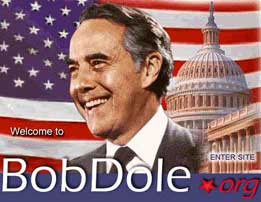
\includegraphics[height=4cm]{bobdole_org.jpg}
            \\ Bob
            %\scalebox{.575}{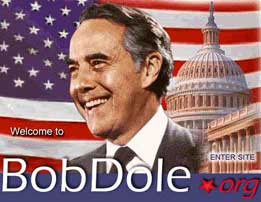
\includegraphics{bobdole_org.jpg}}
        \end{column}
    \end{columns}
    \vspace{10pt}
    \visible<3->{Alice wants to donate \$25 to Bob's campaign}
\end{frame}
\begin{frame}{An illustration}
%    \begin{centering}
    Alice gives Bob a check for \$25 dollars from East Podunk Savings and
    Loan. Bob deposits the check.
    \begin{figure}
        
\includegraphics[height=5cm]{bank}
        \\ East Podunk Savings and Loan
    \end{figure}
%    \end{centering}
\end{frame}

\begin{frame}{An illustration}
    East Podunk S \& L now has a process they need to follow:
    \begin{columns}[t]
        \begin{column}{0.45\textwidth}
            \begin{enumerate}
                \item Take Alice's check from the pile of checks
                \item Debit Alice \$25
                \item Credit Bob \$25
                \item Mark check as processed
                \item Return check to Alice
            \end{enumerate}
        \end{column}
        \begin{column}<2->{0.45\textwidth}
            \color[rgb]{1,0,0}What if...
            \begin{itemize}
                \item     \color[rgb]{1,0,0} \textit{...the server crashes?}
                \item<3-> \color[rgb]{1,0,0} \textit{...step \#1 gets interrupted? (Race condition)}
                \item<4-> \color[rgb]{1,0,0} \textit{...a concurrent process overdraws Alice's account?}
            \end{itemize}
        \end{column}
    \end{columns}
\end{frame}

\begin{frame}{Grouped operations}
    Operations are grouped, and succeed or fail as a group. Groups are called "transactions"

    \begin{itemize}
        \item \textbf{BEGIN} -- Begin a group
        \item \textbf{COMMIT} -- Complete a group
        \item \textbf{ROLLBACK} -- Undo this group
    \end{itemize}
\end{frame}

\begin{frame}{ACID}
    Four characteristics of transactions ("\textbf{ACID}"):
    \begin{itemize}
        \item \textbf{Atomicity} -- Transactions succeed or fail entirely, not partially
        \item \textbf{Consistency} -- After each COMMIT or ROLLBACK, all active database constraints are met
        \item \textbf{Isolation} -- One transaction cannont see uncommited data from any other transaction
        \item \textbf{Durability} -- Once committed, data remain committed despite crashes
    \end{itemize}
\end{frame}

%\begin{frame}{Constraints}
%    Several types are possible:
%    \begin{itemize}
%        \item NOT NULL
%        \item Foreign key
%        \item Check constraints
%        \item Exclusion constraints (PostgreSQL only)
%    \end{itemize}
%\end{frame}

\begin{frame}{NoSQL?}
    In recent years, database users have begun to question the universal
    application of ACID, such as with the NoSQL movement.
    \begin{itemize}
        \item This is not a bad thing
        \item Many applications don't need transactions, ACID
        \item Many more applications still do require transactions and ACID
    \end{itemize}
\end{frame}

\begin{frame}
    True or False: I'm not a bank. Therefore, I don't need transactions.
    \visible<2->{\color[rgb]{1,0,0} \par \vspace{15pt} \textit{False}}
\end{frame}

\begin{frame}{When...}
    Transactions are important...
    \begin{itemize}
        \item When one logical operation requires multiple actual operations
        \item To ensure failures leave you in a known state
        \item If your server might possibly crash
        \item When you have special feelings toward this copy of your data
    \end{itemize}
\end{frame}

\begin{frame}{More examples}
    One End Point client manages call center data. Their application includes
    tasks like these:
    \begin{itemize}
        \item Update notes for a support case
        \item Modify employee performance statistics
        \item Update training databases
        \item Bill customers
    \end{itemize}
    \vspace{10pt}
    Working without transactional guarantees will lead to orphaned records,
    missing information, and irritated customers.
\end{frame}

\begin{frame}{Examples from End Point's clients}
    TriSano\texttrademark  (http://www.trisano.org) is a public health
    reporting application. For each new case, the application can record some
    or all of the following:
    \begin{itemize}
        \item Patient demographics
        \item Participating physicians
        \item Laboratory tests
        \item Reports to various agencies
        \item Contacts of different types
        \item Custom data collection forms
    \end{itemize}
    Data operations touch many tables. Changes need to be atomic to
    prevent orphaned data and ensure consistency.
\end{frame}

\begin{frame}{ORMs}
    \begin{itemize}
        \item Object-Relational Mappers (ORMs) often provide transaction APIs
        \item Users generally ignore those APIs, and use ORM defaults
        \item This behavior is generally wrong
    \end{itemize}
\end{frame}

\begin{frame}
    \frametitle{Rules of thumb}
    \begin{enumerate}
        \item Transactions group operations logically
        \item Only the programmer knows what groupings are logical
    \end{enumerate}
\textit{Ergo}, the programmer should control transactions (not the ORM, the database system, the database driver, or anything else)
\end{frame}

\begin{frame}
    \frametitle{Rules of thumb}
    To decide where to put transaction boundaries:
    \begin{itemize}
        \item Consider units of a business process (``make a sale'') or an application process (``render a web page'')
        \item Consider what operations depend on other related operations in order to make sense
        \begin{itemize}
            \item Don't add this new address unless the associated customer also gets added
            \item Decrease a product's inventory count only if the customer has the money to pay for it
        \end{itemize}
    \end{itemize}
\end{frame}

\begin{frame}
    \frametitle{Rules of thumb}
    You probably need transactions:
    \begin{itemize}
        \item Whether you're ready to admit it or not
        \item Whether you're ready to write your software to handle it or not
        \item If the application has units of work it needs to keep atomic
        \item If the servers might ever crash
        \item Even if your ORM disagrees
    \end{itemize}
\end{frame}

\begin{frame}
    \begin{centering}
        \textbf{Neat Transaction Tricks}
        \par
    \end{centering}
\end{frame}

\begin{frame}{Savepoints}
    Transactions group operations. Within those groups, there may be nested
    subgroups, called subtransactions, implemented with \textbf{savepoints}.
\end{frame}

\begin{frame}{Savepoint Example}
\ttfamily {
\textbf{BEGIN}; \\
\hspace{15pt}\textit{\textendash\textendash\hspace{2pt} Do something useful} \\
INSERT INTO actions VALUES \\
\hspace{10pt} ('IM IN YR AKSHUNZ DOIN YOOSFL STUFS'); \\
\textbf{SAVEPOINT} try\_something; \\
SELECT COUNT(*) FROM some\_other\_table; \\
UPDATE foo SET bar = baz WHERE qux = 42; \\
\hspace{15pt}\textit{\textendash\textendash\hspace{2pt} Pretend there's a constraint error here} \\
\textbf{ROLLBACK TO SAVEPOINT} try\_something; \\
\hspace{15pt}\textit{\textendash\textendash\hspace{2pt} My outer transaction is still
in-flight}
    }
\end{frame}

\begin{frame}{Implementation note}
    In PostgreSQL, a statement that generates an error will invalidate
    everything until the next {\ttfamily ROLLBACK} or {\ttfamily ROLLBACK TO
    SAVEPOINT}: \\
    \vspace{10pt}
    \small{
    \ttfamily {
josh=\# BEGIN; \\
BEGIN \\
josh=\# SELECT syntax error; \\
ERROR:  syntax error at or near "error" \\
LINE 1: SELECT syntax error; \\
josh=\# SELECT 1; \\
{\color{red} \textbf{ERROR:  current transaction is aborted, commands ignored until end of
transaction block}} \\
josh=\# ROLLBACK; \\
    }
    }
    \vspace{10pt}
    If your app gets this error, it's a sign you're not paying attention to
    exceptions correctly, and you therefore suck.
\end{frame}

\begin{frame}{Implementation note}
    MySQL, on the other hand, returns an error message for the syntax error,
    but still allows the transaction to commit: \\
    \vspace{10pt}
    \small {
        \ttfamily {
mysql> start transaction; \\
mysql> insert into i values (1); \\
mysql> insert into i values (2); \\
mysql> insert into i values (1); \\
ERROR 1062 (23000): Duplicate entry '1' for key 1 \\
mysql> insert into i values (3); \\
mysql> commit; \\
Query OK, 0 rows affected (0.00 sec) \\
        }
    }
    \vspace{10pt}
    \pause
    Perhaps this behavior irritates you as much as it does me, since it
    ignores the entire purpose of a transaction.
\end{frame}

\begin{frame}{Implementation note}
    Your mileage may vary. Test, and pay attention to return results and error
    messages
\end{frame}

\begin{frame}{Isolation levels}
    \textbf{Isolation}: No uncommitted data from other sessions is ever visible to my session
    \begin{itemize}
        \item \textbf{Dirty read}: A transaction reads data from a
        concurrent uncommitted transaction
        \item \textbf{Nonrepeatable read}: A transaction re-reads data and
        finds another transaction has committed changes to them
        \item \textbf{Phantom read}: A transaction re-executes a query, and
        the set of rows satisfying that query has changed due to some other
        committed transaction.
    \end{itemize}
\end{frame}

\begin{frame}{Isolation levels}
    The SQL standard defines four isolation levels in terms of these
    phenomena: \\
    \vspace{.5cm}
    \begin{tabular}{llll}
        \textbf{Isolation Level} & \textbf{Dirty} &
        \textbf{Non-repeat} & \textbf{Phantom} \\
        Read uncommitted & Yes & Yes & Yes \\
        Read committed & No & Yes & Yes \\
        Repeatable read & No & No & Yes \\
        Serializable & No & No & No
    \end{tabular}
    \vspace{10pt} \par
    Applications can choose an isolation level appropriate for their needs.
    Stricter levels may entail poorer performance.
\end{frame}

\begin{frame}{Beyond the database}
    The ideas of transactions and ACID are not limited to databases. Some other examples: \\

    \begin{itemize}
        \item Message queues
        \item Integration software
        \item Transactional memory systems
    \end{itemize}
\end{frame}

\begin{frame}[Distributed transactions]
    An operation could, conceivably, want to include multiple transaction-aware services in one transaction:
    \begin{itemize}
        \item Read messages from a queue, and do work in a database in response to those messages
        \item Use data from multiple separate databases
        \item Move messages from one messaging service to another
        \item Build documents using data in a database in a multi-step integration process
    \end{itemize}
    This is possible with \textbf{distributed transactions}
\end{frame}

\begin{frame}
    \frametitle{Two\textendash phase commit}
    A \textit{distributed transaction} is a transaction involving multiple services. It works as follows:
    \begin{enumerate}
        \item BEGIN the transaction in each service
        \item Perform whatever operations are necessary
        \item PREPARE each transaction for commit
        \begin{itemize}
            \item Until this step, the transaction looks like any other. Here
            each service guarantees that the transaction will commit in the
            future, even if something crashes between now and then.
        \end{itemize}
        \item If any service reports it can't commit, we ROLLBACK each transaction
        \item When all services PREPARE successfully, we COMMIT the transaction on each service
    \end{enumerate}
    This is called \textbf{two-phase commit} (2PC) because commit happens in two steps: PREPARE, and COMMIT.
\end{frame}

\begin{frame}
    \frametitle{Two\textendash phase commit}
    2PC is slower than single-phase commit
    \begin{itemize}
        \item On PREPARE, each transaction must store transaction state on
        disk, to ensure durability
        \item The application must also store its own state on disk, in case it
        crashes between PREPARE and COMMIT
        \begin{itemize}
            \item Applications generally use \textit{transaction managers}
            rather than handle these details on their own
        \end{itemize}
    \end{itemize}
\end{frame}

\begin{frame}
    \frametitle{Bitronix transaction manager example}
\footnotesize {
\ttfamily {
\#!/bin/jruby \\
require 'java' \\
\vspace{10pt}
{\color{DodgerBlue} BTM} = {\color{DodgerBlue} Java::BitronixTm::bitronixTransactionManager} \\
{\color{DodgerBlue} TxnSvc} = {\color{DodgerBlue} Java::BitronixTm::TransactionManagerServices} \\
{\color{DodgerBlue} PDS} = {\color{DodgerBlue} Java::BitronixTmResourceJdbc::PoolingDataSource} \\
\vspace{10pt}
{\color{gray} \# Do the stuff below for each data source} \\
ds1 = {\color{DodgerBlue}PDS}.new \\
ds1.set\_class\_name {\color{BlueViolet}'org.postgresql.xa.PGXADataSource'} \\
\textellipsis \\
ds1.init \\
{\color{gray} \# Get datasource connections, and start a transaction} \\
c1 = ds1.get\_connection \\
c2 = ds2.get\_connection \\
btm = {\color{DodgerBlue}TxnSvc}.get\_transaction\_manager \\
btm.begin \\
}
}
\end{frame}

\begin{frame}
    \frametitle{Bitronix transaction manager example}
\footnotesize {
\ttfamily {
{\color{DodgerBlue}\textbf{begin}} \\
\hspace{40pt} \# Do something on each connection \\
\hspace{40pt} s2 = c2.prepare\_statement \\
\hspace{80pt} {\color{BlueViolet}"INSERT INTO ledger VALUES ('Bob', 100)"} \\
\hspace{40pt} s2.execute\_update \\
\hspace{40pt} s2.close \\
\hspace{40pt}  \textellipsis \\
\hspace{40pt}  btm.commit \\
\hspace{40pt}  puts {\color{BlueViolet}"Successfully committed"} \\
{\color{DodgerBlue}\textbf{rescue }}\\
\hspace{40pt}  puts {\color{BlueViolet}"Something bad happened: "} + \$! \\
\hspace{40pt}  btm.rollback \\
{\color{DodgerBlue}\textbf{end }}\\
}}
\end{frame}

\begin{frame}
    \begin{centering}
\textbf{Transaction pitfalls}
    \par
    \end{centering}
\end{frame}

\begin{frame}
    \frametitle{Stuff to watch out for}
    \begin{itemize}
        \item Long transactions are typically bad
        \begin{itemize}
            \item Locks remain held until transactions commit
            \item Rollback space can't be released until commit
            \item This may be particularly bad with 2PC
            \item Note that in PostgreSQL, \textbf{everything} happens within a transaction
            \begin{itemize}
                \item You don't have to explicitly begin the transaction, but
                you \textbf{do} have to explicitly close them, if you turn off
                ``AutoCommit''
                \item If you don't, they'll become one of these evil long transactions
            \end{itemize}
        \end{itemize}
        \item More complex transactions are probably more likely to roll back
        \item Handle exceptions properly (you're doing this already, right?)
        \begin{itemize}
            \item If you roll back and try again, you have to redo the entire operation
        \end{itemize}
    \end{itemize}
\end{frame}

\begin{frame}
    \begin{centering}
\textbf{Transaction benefits}
    \par
    \end{centering}
\end{frame}

\begin{frame}
    \frametitle{Miscellaneous transaction benefits}
    \begin{itemize}
        \item Performance
        \begin{itemize}
            \item For example, several INSERTs in their own transactions will
            be slower than the same INSERTs grouped into one transaction.
        \end{itemize}
        \item Simpler code
        \begin{itemize}
            \item Wrap one transaction in one exception handling block
        \end{itemize}
        \item Data integrity
        \begin{itemize}
            \item Orphaned records and other data anomalies are much less likely
        \end{itemize}
    \end{itemize}
\end{frame}

\begin{frame}
    \begin{centering}
        \textbf{Questions?} \par
    \end{centering}
\end{frame}

% - You need transactions whether you're ready to admit it or not
% - The application has units of work it needs to keep atomic. What's more, only the application knows the boundaries of those units
% - Unfortunately often your ORM disagrees with these last two

% - Lots of programmers are too lazy to catch and handle transaction errors (e.g. locking failures, serialization failures)
% - Some people understand transactions' importance enough to transaction-enable other stuff. Message queues, data transformation services
% Multiple transactional systems can coordinate via 2PC
% - Java has the XA spec, and transaction managers. Federation software is also a possibility
% - There aren't many non-Java transaction managers
% - You can have one (but not more) non-2PC capable devices in a commit group, if it's done right
% Problems with pathological behavior
% - Locking tons of stuff
% - Long transactions are bad, and not just because of PostgreSQL and vacuum
% - Serialization failures
% What to do about it all?... 

% A story:

% Alice is building a web application to sell widgets, and needs a database. Part
% of the database needs to store customer names. Her database has data types for
% "text", and length-constrained "varchar". She prefers a length constraint,
% because she's heard TEXT can be slow, and she doesn't want people to enter a 2
% GB name anyway. She doesn't know how big to make it, but she figures it has to
% be a power of two, because that seems like what everyone does. So how about 64
% characters? Or should it be a power of two minus one? 63? Ok, so customer_name
% VARCHAR(63). This is all fine and good, but how did we choose that limit? Oh,
% right, it was fairly random. Do the developers know about it? Erm... So if
% something fails because a user actually entered a 2 GB name, will the code
% notice?
%
%Note:
%PostgreSQL's tendency to yell when you freak out a transaction, and keep
%yelling, is a good thing. That makes it harder for bad programmers to fail to
%note they've had an error. It means once something has gone wrong, and part of
%the transaction has failed, it means the rest of the transaction will always
%fail It means once something has gone wrong, and part of teh transaction has
%failed, it means the rest of the transaction will always fail. Whcih is the
%point of transactions
%
%Ok, now I have some database constraints, which means I'm Doing It Right. 
%But if you don't have all this in a strict transaction, you'll have some of the
%data commit, and some of it not commit. 
%
%Users can sometimes figure out when stuff like this happens, and deal with the
%results, but this gets particularly irritating when the new Management
%Consultant comes in with a report that the automated web app testing service
%isn't getting repeatable results.

\end{document}
